\documentclass{article}

\usepackage[paperwidth=5.5in, paperheight=8.5in, top=0.8in, bottom=0.8in, inner=0.8in, outer=0.8in]{geometry}

\usepackage{caption}
\usepackage{subcaption}
\usepackage{graphicx}
\usepackage{svg}
\usepackage[utf8]{inputenc}

\usepackage[colorlinks=true]{hyperref}

\usepackage{endnotes}
\let\footnote=\endnote

\usepackage{ulem}
\usepackage[outline]{contour}
\newcommand \myul[4]{%
  \begingroup%
  \renewcommand \ULdepth {#1}%
  \renewcommand \ULthickness {#2}%
  \contourlength{#3}%
  \uline{\phantom{#4}}\llap{\contour{white}{#4}}%
  \endgroup%
}

\newcommand \myulline[4]{%
  \begingroup%
  \renewcommand \ULdepth {#1}%
  \renewcommand \ULthickness {#2}%
  \contourlength{#3}%
  \noindent\rlap{\uline{\hspace{\textwidth}}}\contour{white}{#4}%
  \endgroup%
}

\usepackage{fontspec}
\defaultfontfeatures{Mapping=tex-text,Scale=MatchLowercase}
\setmainfont{Times New Roman}
\setmonofont{IBM Plex Mono}

\newfontfamily\Hiero{Noto Sans Egyptian Hieroglyphs}
% \newcommand*{\hieroglyphics}{\fontfamily{Noto Sans Egyptian Hieroglyphs}\selectfont}


\begin{document}
\author{James Babcock (jimrandomh@gmail.com)}
\title{Petrov Day}

\newcommand{\divider}{ %{{{
	% From http://tex.stackexchange.com/questions/32711/totally-sweet-horizontal-rules-in-latex
	\nointerlineskip \vspace{\baselineskip}
	\hspace{\fill}\rule{0.5\linewidth}{.7pt}\hspace{\fill}
	\par\nointerlineskip \vspace{\baselineskip}
} %}}}
\newcommand{\stagedir} [1] { %{{{
	\begin{itshape}
	#1
	\end{itshape}
} %}}}
\newcommand{\blockquote} [2] { %{{{
	\begin{center}
		\parbox{3.5in}{
			``#1''
			\begin{flushright}
				--- #2
			\end{flushright}
		}
	\end{center}
} %}}}
\newcommand{\blockquoteUnattributed} [1] { %{{{
	\begin{center}
		\parbox{3.5in}{
			``#1''
		}
	\end{center}
} %}}}
\newcommand{\blockspacing} [1] { %{{{
	\begin{center}
		\parbox{3.5in}{
			#1
		}
	\end{center}
} %}}}
\newcommand{\blockquoteUnmarked} [2] { %{{{
	\begin{center}
		\parbox{3.5in}{
			#1
			\begin{flushright}
				--- #2
			\end{flushright}
		}
	\end{center}
} %}}}
\newcommand{\poem} [2] { %{{{
	\begin{center}
		\parbox{3.5in}{
			#1
			\begin{flushright}
				--- #2
			\end{flushright}
		}
	\end{center}
} %}}}
\newcommand{\page} [1] { %{{{
	\divider
	#1
	\divider
	\newpage
} %}}}
\newcommand{\pageNoBottomDiv} [1] { %{{{
	\divider
	#1
	\newpage
} %}}}
\newcommand{\sidePage} [1] { %{{{
	\vspace*{0.2in}
	#1
	\newpage
} %}}}
\newcommand{\candelabrum} [1] { %{{{
	\begin{center}
		\includegraphics[width=3in]{#1}
	\end{center}
} %}}}
\newcommand{\candlePassing} { %{{{
	\begin{center}
		\includegraphics[width=2.5in]{images/candlepassing.png}
	\end{center}
} %}}}

% Don't indent paragraphs
\setlength{\parindent}{0cm}

\setlength{\parskip}{\baselineskip}

%%%%%%%%%%%%%%%%%%%%%%%%%%%%%%%%%%%%%%%%%%%%%%%%%%%%%%%%%%%%%%%%%%%%%%

% Front Matter
% Title page {{{
\pagenumbering{gobble}
\sidePage{

\begin{flushright}
\parbox{3in}{
	\begin{center}
		\Huge{Petrov Day}\newline
		\large{September 26th}\newline
		By Austin Ritual Working Group\newline
	\end{center}
}
\end{flushright}

}

\pagenumbering{arabic}
\page{

Set up a \myul{2pt}{0.5pt}{1pt}{table} in the middle of the room and gather everyone around.

Place on the table:
\begin{itemize} \itemsep0pt \parskip0pt \parsep0pt
	\item a \myul{2pt}{0.5pt}{1pt}{candelabrum} with eight holders,
	\item \myul{2pt}{0.5pt}{1pt}{seven unlit candles} in a
	\myul{2pt}{0.5pt}{1pt}{tray} (but not in the candelabrum), and
	\item a \myul{2pt}{0.5pt}{1pt}{lighter or matches} (and if the latter,
	\myul{2pt}{0.5pt}{1pt}{a cup of sand or water} in which to douse them).
\end{itemize}

Take an \myul{2pt}{0.5pt}{1pt}{eighth candle} and insert it into a
\myul{2pt}{0.5pt}{1pt}{candle-holder} so that it can be moved around without
dripping wax. Have a \myul{2pt}{0.5pt}{1pt}{printed copy}
\myul{2pt}{0.5pt}{1pt}{of this booklet} ready.

The ceremony should begin after dark. Start with the lights on or dimmed, but
turn them off once the first candle is lit.

}

\page{

\stagedir{The speech should be given extemporaneously, but make sure to cover
all the bullet points.}

Welcome to the Petrov Day ceremony. Here's how it works:

\begin{itemize} \itemsep0pt \parskip0pt \parsep0pt
	\item We will pass around this booklet, and take turns reading from it by
	candlelight.
	\item When it comes to you, read aloud the text in bold and do the actions
	described in brackets.
	\item Speak loudly and clearly, so everyone can hear you. Don’t worry about
	hard-to-pronounce words; just power through them.
	\item When reading quotes, read the attribution at the end.
	\item If you see a triangle symbol (▲), come up to the table and
	perform the action.
	\item When you come to a horizontal line, pass the booklet and candle
	to the next person.
	\item Please silence your phones.
\end{itemize}

Are there any questions?\stagedir{Pause for questions}

Let us begin.

}

\page{

This day, September 26th, is Petrov Day.

\rule{0.8cm}{0.15mm} \textit{(years since 1983)} years ago today, the story of
humanity nearly ended. We gather here to remember that moment, and others like
it.

\poem{That not a worm is cloven in vain;\newline
	That not a moth with vain desire\newline
	Is shriveled in a fruitless fire,\newline
	Or but subserves another's gain.\newline
	\newline
	Behold, we know not anything;\newline
	I can but trust that good shall fall\newline
	At last—far off—at last, to all,\newline
	And every winter change to spring.\newline
	\newline
	So runs my dream: but what am I?\newline
	An infant crying in the night:\newline
	An infant crying for the light:\newline
	And with no language but a cry.}{In Memoriam A.H.H., Alfred Lord Tennyson
	(1850)}

} %}}}
% Prometheus quote: Light candle 1 {{{
\page{

\stagedir{▲ Light the candle in the candle-holder with a match or
lighter, hold it high, and say:}

The first candle, for fire.

\divider

\poem{
	Ναρθηκοπληρωτον δε θηρωμαι πυρος\newline
	Πηγην κλοπαιαν, η διδασκαλος τεχνης\newline
	Πασης βροτοις πεφηνε και μεγας πορος.\newline
	Τοιωνδε ποινας αμπλακηματων τινω\newline
	Υπαιθριος δεσμοις πεπασσαλευμενος.\newline

	I sought the fount of fire in hollow reed\newline
	Hid privily, a measureless resource\newline
	For man, and mighty teacher of all arts.\newline
	This is the crime that I must expiate\newline
	Hung here in chains, nailed 'neath the open sky.\newline}
{Prometheus Bound, Aeschylus (c. 450 BC)\footnote{\href{
	https://web.archive.org/web/20090107185646/
	http://etext.library.adelaide.edu.au/a/aeschylus/prometheus/}{
		http://etext.library.adelaide.edu.au/a/aeschylus/prometheus/}}}

}

\sidePage {

\newcommand{\skull} [2] { %{{{
	\parbox{1.3in}{
		\begin{center}
			\includegraphics[width=1.2in]{#1}
			#2
		\end{center}
	}
} %}}}

\skull{images/H_ergaster.png}{\textit{Homo ergaster}}
\skull{images/H_erectus.png}{\textit{Homo erectus}}
\skull{images/H_floresiensis.png}{\textit{Homo floresiensis}}
\skull{images/H_habilis.png}{\textit{Homo habilis}}
\skull{images/H_heidelbergensis.png}{\textit{Homo heidelbergensis}}
\skull{images/H_neanderthalensis.png}{\textit{Homo neanderthalensis}}
\skull{images/H_rudolfensis.png}{\textit{Homo rudolfensis}}

}

\page {

\candelabrum{images/candelabrum_2.png}

\stagedir{▲ Remove the lit candle from the holder and place it in the
first slot of the candelabrum.

Place an unlit candle in the holder.

Light this candle from the one in the candelabrum and hold it high, saying:}

The second candle, for language.

\divider

\blockquote{It certainly is not a true instinct, for every language has to be
learnt. It differs, however, widely from all ordinary arts, for man has an
instinctive tendency to speak, as we see in the babble of our young children;
whilst no child has an instinctive tendency to brew, bake, or write.}{Charles
Darwin, Descent of Man (1871)}

}

\pageNoBottomDiv{

\candelabrum{images/candelabrum_3.png}

\stagedir{▲ Remove the lit candle from the holder and place it in the second
slot of the candelabrum.

Place an unlit candle in the holder.

Light this candle from the one in the second slot of the candelabrum and hold
it high, saying:}

The third candle, for farming.

\divider

\blockquote{
ἆρ᾽ οὖν ὑμῖν οἱ παλαιοὶ λόγοι ἀλήθειαν ἔχειν τινὰ δοκοῦσιν; [...] τὸ πολλὰς
ἀνθρώπων φθορὰς γεγονέναι κατακλυσμοῖς τε καὶ νόσοις καὶ ἄλλοις πολλοῖς, ἐν
οἷς βραχύ τι τῶν ἀνθρώπων λείπεσθαι γένος. - πάνυ μὲν οὖν πιθανὸν τὸ
τοιοῦτον πᾶν παντί. - φέρε δή, νοήσωμεν μίαν τῶν πολλῶν ταύτην τὴν τῷ
κατακλυσμῷ ποτε γενομένην.\newline

Do you believe that there is any truth in ancient traditions [...] about the
many destructions of mankind which have been occasioned by deluges and
pestilences, and in many other ways, and of the survival of a remnant? ---
Every one is disposed to believe them. --- Let us consider one of them, that
which was caused by the famous deluge.}{Laws, Plato (c. 350 BC)\footnote{
	Greek: \href{https://www.perseus.tufts.edu/hopper/text?doc=Plat.+Laws+3.677
		\&fromdoc=Perseus\%3Atext\%3A1999.01.0165}{
			https://www.perseus.tufts.edu/hopper/text?doc=Plat.+Laws+3.677
			\&fromdoc=Perseus\%3Atext\%3A1999.01.0165}\newline
	English: \href{https://en.wikisource.org/wiki/Laws\_(Jowett)/Book\_III}{
		https://en.wikisource.org/wiki/Laws\_(Jowett)/Book\_III}\newline
	source for date: \href{https://www.csun.edu/~hcfll004/platochron.html}{
		https://www.csun.edu/~hcfll004/platochron.html}}
}

}

\page{

\stagedir{▲ Extinguish the candle in the holder.}

Humanity lived in a delicate balance of knowledge gained and forgotten,
relying solely on memory and oral traditions. With the advent of writing, the
preservation of knowledge expanded, and the equilibrium between learning and
forgetting was broken.

\stagedir{Light the candle in the holder again from the one in the
second slot of the candelabrum, and hold it high, saying:}

The third candle again, for writing.

\divider

\begin{center}
	\includesvg[width=3.5in]{images/rosetta_hieroglyphics.svg}
\end{center}

\blockquote{%{\Hiero [...]𓋴𓆼𓏲𓏭𓀁𓊪𓏌𓁷𓏤𓊢𓂝𓇌𓏏𓈖𓏏𓏭𓉻𓏏𓈜𓌗𓐝𓏟𓈖𓊹𓌃𓏪𓏟𓋔𓈚𓂝𓇌𓌪𓋴𓆼𓇌𓌪𓋔𓇇𓏲𓏭𓎠𓎠𓀀𓏪𓂋𓏏𓂝𓊢𓂝𓂻𓆑𓅓𓊸𓊸𓊸
%𓐝𓂋𓏥𓉔𓊖𓎠𓁷𓏤𓍷𓀋𓄱𓏤𓎖𓏺𓎖𓏻𓎖𓏼𓂋𓐝𓏤𓂙𓏌𓏤𓀙𓋔𓆥𓍹𓊪𓏏𓍯𓃭𓐝𓇌𓋴𓋹𓆓𓏏𓇾𓊪𓏏𓎛𓌹𓇌𓍺𓊹𓉔𓂋𓂻𓎠𓄤𓄤𓄤}
[...]ΤΕΡΟΥ ΛΙΘΟΥ ΤΟΙΣ ΤΕ ΙΕΡΟΙΣ ΚΑΙ ΕΓΧΩΡΙΟΙΣ ΚΑΙ ΕΛΛΗΝΙΚΟΙΣ ΓΡΑΜΜΑΣΙΝ ΚΑΙ
ΣΤΗΣΑΙ ΕΝ ΕΚΑΣΤΩΙ ΤΩΝ ΤΕ ΠΡΩΤΩΝ ΚΑΙ ΔΕΥΤΕΡΩ[...]\newline

This decree [shall be inscribed] on a tablet of hard stone in hieroglyphic,
demotic, and Greek writing and set up in each of the temples of the first,
second, and third rank beside the image of the King
\myul{2pt}{0.5pt}{1pt}{Ptolemy, ever-living, beloved of Ptah}, the god manifest,
lord of good deeds.}{Rosetta Stone (c. 196 BC)\footnote{Budge, E.A. Wallis.
(1929). The Rosetta Stone in the British Museum (pp. 168–9). The Religious Tract
Society.}}

}

\sidePage{

\includegraphics[width=4in]{images/RosettaStone.png}

}

\page{

While much writing took the form of legal codes, genealogies, and other
everyday matters, some of it advanced our knowledge of the world---and more
importantly, our method for finding it.

\divider

\candelabrum{images/candelabrum_4.png}

\stagedir{▲ Remove the lit candle from the holder and place it in the
third slot of the candelabrum.

Place an unlit candle in the holder.

Light this candle by touching it in turn to the three lit candles, and hold it
high, saying:}

The fourth candle, for science.

}

\page{

\blockquote{\textit{Qui ergo vult sine demonstratione gaudere de veritatibus
rerum, oportet quod experientiae sciat vacare; et hoc patet ex exemplis. Nam
multa scribunt auctores, et vulgus tenet per argumenta quae fingit sine
experientia, quae sunt omnino falsa.}\newline

He therefore who wishes to rejoice without doubt in regard to the truths
underlying phenomena must know how to devote himself to experiment. For authors
write many statements, and people believe them through reasoning which they
formulate without experience. Their reasoning is wholly false.}{Roger Bacon,
Opus Majus (1266) \footnote{
\href{https://archive.org/details/opusmajusofroger02bacouoft/page/168/mode/2up}{
Latin text}: Bridges, Henry, ed. (1898). The 'Opus Majus' of Roger Bacon (vol.
2, p. 168). Clarendon press.} \footnote{
\href{https://archive.org/details/opusmajusofroger002065mbp/page/n183/mode/2up}{
English translation}: Burke, Robert Belle, trans. (1962). The Opus Majus of
Roger Bacon (vol. 2, p. 584). Russell \& Russell Inc.}}

\divider

\candelabrum{images/candelabrum_5.png}

\stagedir{▲ Remove the lit candle from the holder and place it in the
fourth slot of the candelabrum.

Place an unlit candle in the holder.

Light this candle from the one you just placed in the candelabrum and hold it
high, saying:}

The fifth candle, for industry.

}

\page{

\blockquote{[...] it may become possible to set up a nuclear chain reaction in
a large mass of uranium, by which vast amounts of power and large quantities
of new radium-like elements would be generated. Now it appears almost certain
that this could be achieved in the immediate future.\newline

This new phenomenon would also lead to the construction of bombs, and it is
conceivable—though much less certain—that extremely powerful bombs of a new
type may thus be constructed.}{Einstein/Szilard Letter (August 2, 1939)}

\divider

Meanwhile, the rockets that had first been developed for war were
turned to exploration as well:

\blockquote{Here men from the planet Earth first set foot upon the Moon July
1969, A.D. We came in peace for all mankind}{Plaque left on the Moon by Apollo
11 astronauts (1969)}

}

\sidePage{

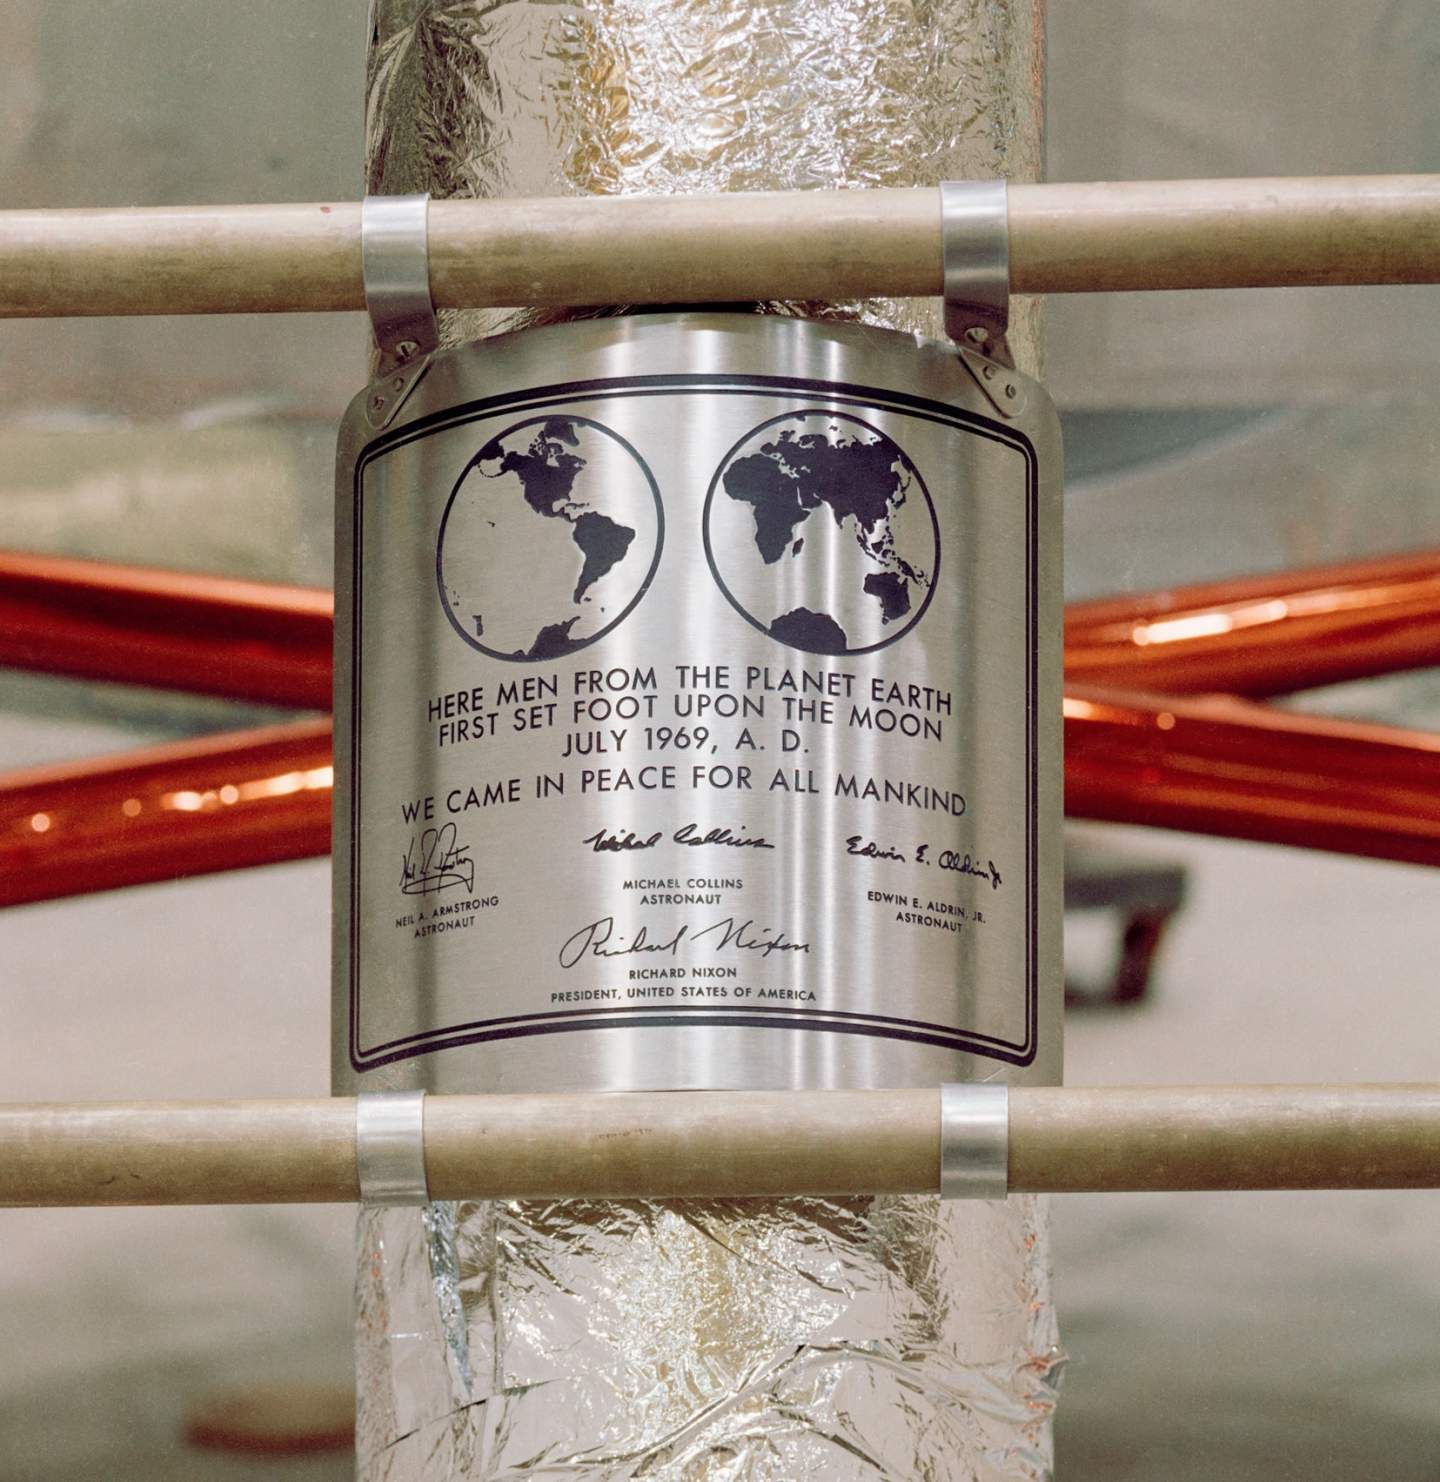
\includegraphics[width=4in]{images/apollo_11_plaque.jpg}

}

\pageNoBottomDiv{

\candelabrum{images/candelabrum_6.png}

\stagedir{▲ Remove the lit candle from the holder and place it in the
fifth slot of the candelabrum.

Place an unlit candle in the holder.

Light this candle from the one you just placed in the candelabrum and hold it
high, saying:}

The sixth candle, for computing.

\divider

\blockquote{Let an ultraintelligent machine be defined as a machine that can
far surpass all the intellectual activities of any man however clever.\newline

Since the design of machines is one of these intellectual activities, an
ultra-intelligent machine could design even better machines; there would then
unquestionably be an ``intelligence explosion,'' and the intelligence of man
would be left far behind.\newline

Thus the first ultraintelligent machine is the last invention that man need ever
make, provided that the machine is docile enough to tell us how to keep it under
control.}{I. J. Good, Speculations Concerning the First Ultraintelligent Machine
(1963)}

}

\page{

\candelabrum{images/candelabrum_6_unlit_1.png}

\stagedir{▲ Set the candle-holder down on the table. Take an unlit
candle and hold it high, saying:}

The seventh candle, for a flourishing future.

\stagedir{Place the candle, still unlit, in the last slot of the candelabrum.
Take the candle-holder with the lit candle back to your seat, and pass it and
the booklet along.}

\divider

On September 26th, 1983, Stanislav Petrov was the duty officer at the Oko
nuclear early warning system.

}

\page{

\blockquote{Сирена на КП вовсю ревет, красные буквы полыхают. Шок, конечно,
колоссальный. [...] Все повскакивали из-за пультов, на меня смотрят. А я что?
Все по инструкции для оперативных дежурных, которую сам и написал. Сделали
все, что нужно. Проверили функционирование всех систем. Тридцать уровней
проверки, один за другим. Идут доклады: все совпадает, вероятность - двойка.
[...] Это высшая[.]\newline

An alarm at the command and control post went off with red letters blinking on
the terminal. It was a nasty shock. Everyone jumped from their seats, looking at
me. What could I do? There was an operations procedure that I had written
myself. We did what we had to do. We checked the operation of all systems—on 30
levels, one after another. Reports kept coming in: All is correct; the
probability factor is two. ... The highest.}{Stanislav
Petrov\footnote{\href{https://web.archive.org/web/20130629104257/
http://flb.ru/info/27637.html}{http://flb.ru/info/27637.html}}}

\begin{center}
	\includegraphics[width=3.0in]{images/StanislavPetrov.jpg}
\end{center}

}

\page{

The procedure was clear: report up the chain of command that the Americans had
launched missiles. This could have set off a nuclear war.

If the launch was real, failing to report it promptly could mean losing a
nuclear war.

What would you have done?

\divider

\blockquote{If you say why not bomb them tomorrow, I say why not today? If you
say today at 5 o'clock, I say why not one o'clock?}{John von Neumann
(1950)\footnote{Poundstone, W. (1993). Prisoner’s Dilemma: John von Neumann,
Game Theory, and the Puzzle of the Bomb (p. 4). Anchor Books.}}

\blockquote{I imagined if I’d assume the responsibility for unleashing the third
World War—and I said, no, I wouldn’t. ... I always thought of it. Whenever I
came on duty, I always refreshed it in my memory.}{Stanislav
Petrov\footnote{\href{https://web.archive.org/web/20040610193448/
http://www.mosnews.com/feature/2004/05/21/petrov.shtml}{
	http://www.mosnews.com/feature/2004/05/21/petrov.shtml}}}

\divider

Instead of telling his superiors what the system was saying, Petrov told his
superiors that it was a false alarm---despite not really knowing this was the
case.

}

\page{

At the time, he received no award. The incident embarrassed his superiors and
the scientists responsible for the system, so if he had been rewarded, they
would have had to be punished. (He received the International Peace Prize
thirty years later, in 2013).

\divider

Things eventually calmed down. The Soviet Union dissolved. Safeguards were put
on most bombs, to prevent the risk of accidental (or deliberate but
unauthorized) detonation.

But not every threat to humanity is as easy to understand as nuclear weapons.

\divider

\blockquote{The AI does not hate you, nor does it love you, but you are made
out of atoms which it can use for something else. The AI runs on a different
timescale than you do; by the time your neurons finish thinking the words ``I
should do something'' you have already lost.}{Eliezer Yudkowsky, Artificial
Intelligence as a Positive and Negative Factor in Global Risk (2006)}

}

\page{

\candelabrum{images/candelabrum_6_unlit_2.png}

\stagedir{▲ Set the candle-holder down on the table. Take an unlit
candle and hold it high, saying:}

Another seventh candle, for an empty future.

\stagedir{Place the candle, still unlit, in the last slot of the candelabrum.
Take the candle-holder with the lit candle back to your seat, and pass it and
the booklet along.}

\divider

On September 7th, 2017, a friend of Stanislav Petrov called him on the phone to
wish him a happy birthday, only to learn that he had died several months
prior, in May of that year.

}

\page{

\candelabrum{images/candelabrum_6_unlit_2_in_hand.png}

\stagedir{Remove the lit candle from the holder and place it in the sixth slot
of the candelabrum.

Lay the booklet flat on the table.

Take the two unlit candles from the candelabrum and hold them close to the flame
of the candle you just placed in the candelabrum.}

Which brings us at last to the present day, as we approach the climax of our
history, where we will either destroy ourselves, or spread through the stars.

\stagedir{Return the unlit candles to the candelabrum, take the booklet back
to your seat, and pass it along.}

}

\page{

After each of the six invocations, when the candle is raised, repeat together
``We will remember''. After the seventh, repeat ``So say we all''.

\divider

\begin{center}
	
\includegraphics[width=1.0in]{images/candle_1_fire.png}
\end{center}

\stagedir{▲ Take the first candle from the candelabrum.}

With fire, we become free from darkness, free from fear of the beasts of the
night, and free to give thought to the times ahead.

That we can make light, even in the darkest times---

\stagedir{Raise the candle high.}

---we will remember.

\textit{(All):} We will remember.

}

\page{

\begin{center}
	
\includegraphics[width=1.25in]{images/candle_2_speech.png}
\end{center}

\stagedir{▲ Take the second candle from the candelabrum.}

With speech, our minds grow beyond us and between us. We can share what we know,
and learn the thoughts and feelings of others.

That we can learn and teach---

\stagedir{Raise the candle high.}

---we will remember.

\textit{(All):} We will remember.

}

\page{

\begin{center}
	
\includegraphics[width=1.25in]{images/candle_3_writing.png}
\end{center}

\stagedir{▲ Take the third candle from the candelabrum.}

With writing, we take on the wisdom of those who came before us. We stand upon
the shoulders of giants, and see farther than they did, though we may not be
giants ourselves.

That we have a hoard of knowledge upon which to build---

\stagedir{Raise the candle high.}

---we will remember.

\textit{(All):} We will remember.

}

\page{

\begin{center}
	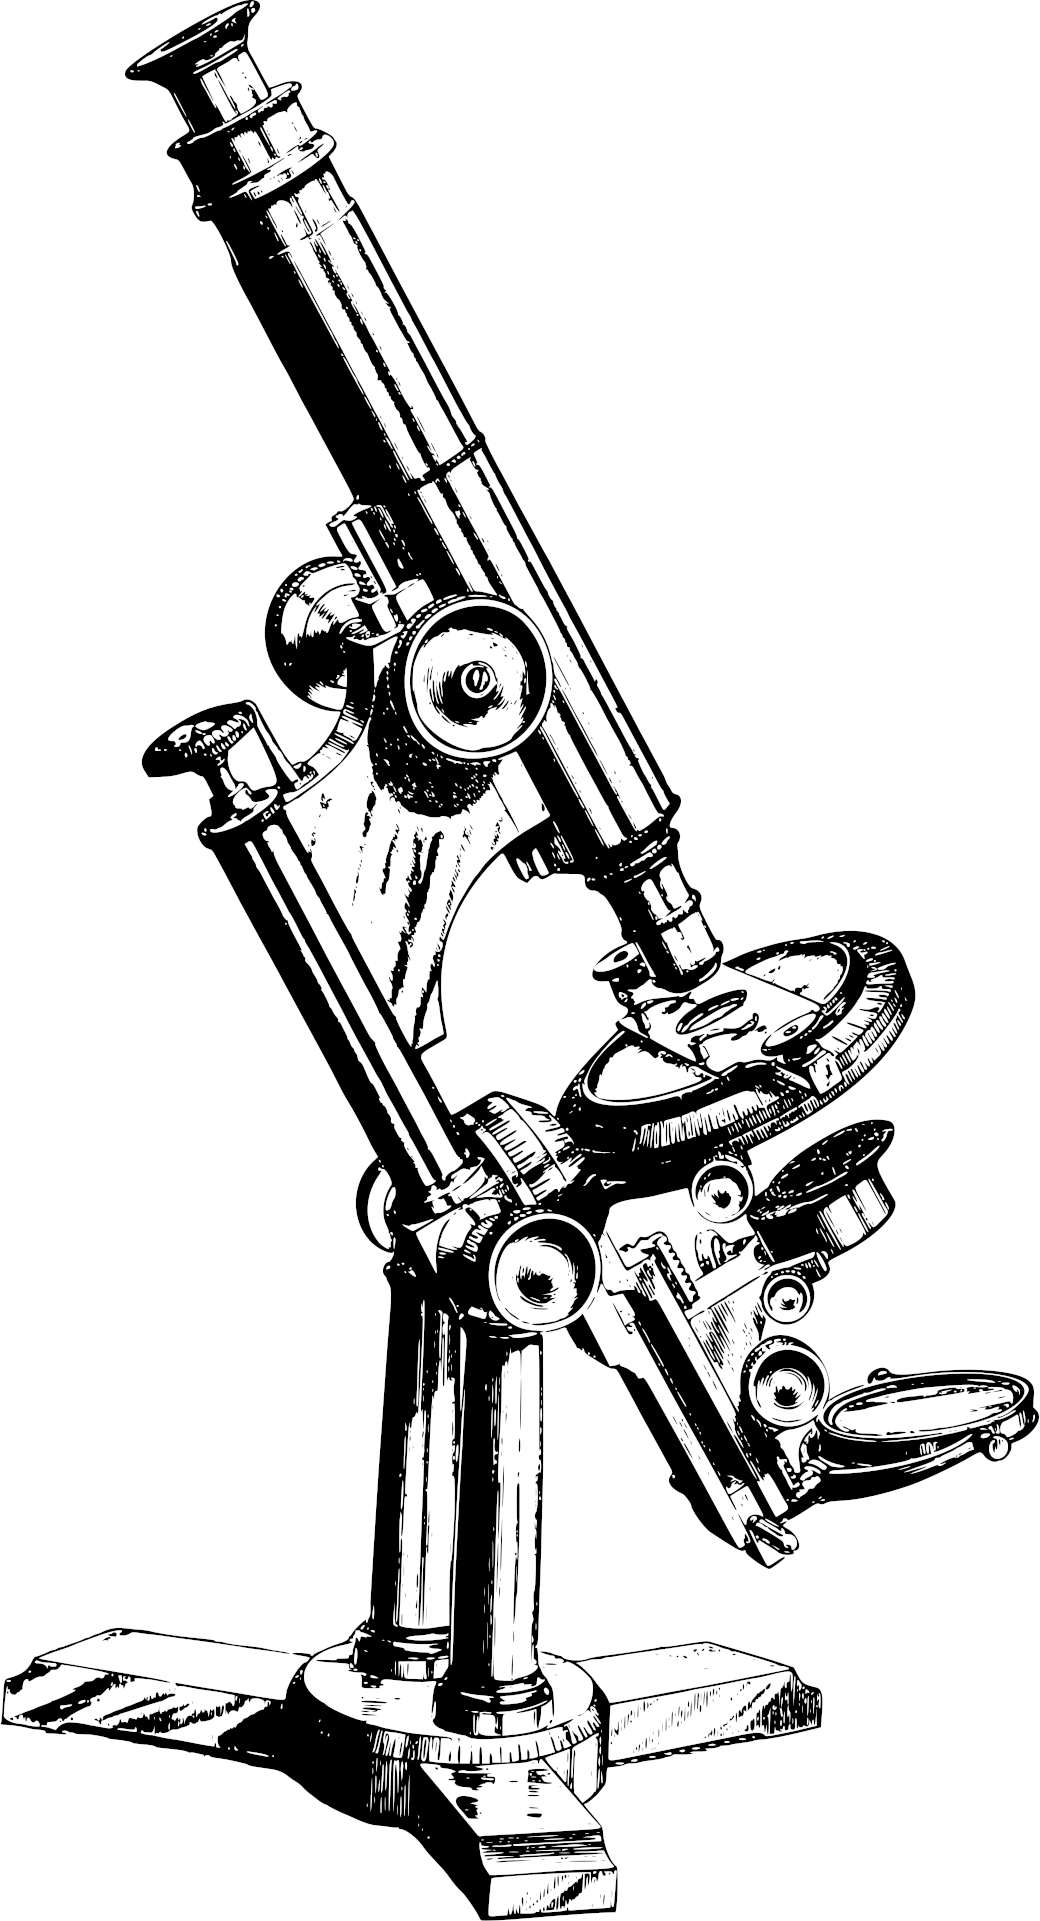
\includegraphics[width=1.25in]{images/candle_4_science.png}
\end{center}

\stagedir{▲ Take the fourth candle from the candelabrum.}

With science, we broach the true nature of a world where physical laws set forth
the outcomes of what we do.

That we can forecast the future, and work to sway its course---

\stagedir{Raise the candle high.}

---we will remember.

\textit{(All):} We will remember.

}

\page{

\begin{center}
	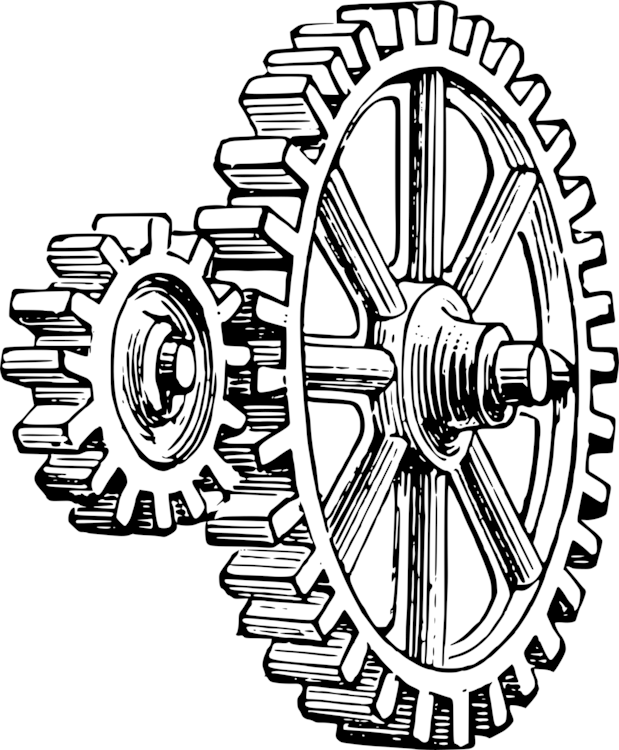
\includegraphics[width=1.25in]{images/candle_5_industry.png}
\end{center}

\stagedir{▲ Take the fifth candle from the candelabrum.}

With industry, the burden of our struggle for survival is lightened. More so
than ever before, we need no longer live hand-to-mouth. Comparative plenty of
food and shelter frees us from having to toil in the fields, and lets us choose
how to live.

That we can turn our thoughts to other, greater things---

\stagedir{Raise the candle high.}

---we will remember.

\textit{(All):} We will remember.

}

\page{

\begin{center}
	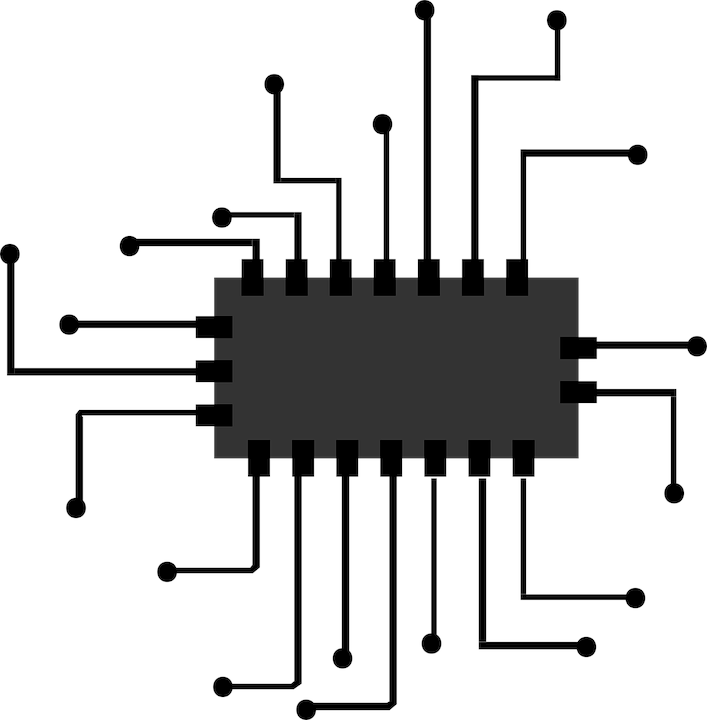
\includegraphics[width=1.25in]{images/candle_6_computing.png}
\end{center}

\stagedir{▲ Take the sixth candle from the candelabrum.}

With computing, our minds are made mighty. Our words fly all over the world. We
behold the fullness of human knowledge, and can search it with a word. Tools
from across the earth are at our fingertips.

That we, the children of computing, are powerful---

\stagedir{Raise the candle high.}

---we will remember.

\textit{(All):} We will remember.

}

\pageNoBottomDiv{

\begin{center}
	
\includegraphics[width=0.5in]{images/candle_7a_flourishing_future.png}
\end{center}

\stagedir{▲ Take the last, unlit candle from the candelabrum.}

Today we gather in the shadow of many dangers. May we one day be free from all
fear, and free for all things to come.

\stagedir{Raise the candle high.}

So say we all.

\textit{(All):} So say we all.

\candelabrum{images/final_candelabrum.png}

\stagedir{Return the candle to the last slot of the candelabrum. Turn on the
lights and then put out the candles. This concludes the ceremony.}

}

\pagenumbering{gobble}

% Rear cover {{{
\sidePage{

\theendnotes

}
% }}}

\end{document}
